\setchapterpreamble[u]{\margintoc}
\chapter{Glossary}

\begin{description}
\item[WYSIWYG] : Which means What You See Is What You Get. You can tell a text editor is WYSIWYG when its edition view is the exact rendering of the final view you will get of the printed document.

\item[RAM] : Rapid Access Memory, it is the specific memory of a computer allowing it to do several things in the shame time without latency.

\item[Templates] : We call template a pre-filled document with frequently requested paragraphs and sections that can be used or erased to ease the exhaustive redaction of a document.

\item[Requirements] : We call requirement the detailed description of an independent item of the project. This item can either be a needs assessment from the customer or a solution feature from the supplier. It is like a brick or a piece of a puzzle.
\begin{figure}[h]
    \centering
    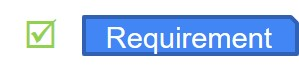
\includegraphics[]{Requirement}
    \caption{A requirement}
    \label{fig:mesh1}
\end{figure}

\item[Coverage] : Imagine a requirement ‘A’ describing an simple need.
We say that the requirement ‘A’ is covered by the requirement ‘B’, if the requirement ‘B’ describes the feature matching the need described by requirement ‘A’. 
\begin{figure}[h]
    \centering
    
\includegraphics[]{exigences-connectees}
    \caption{2 connected requirements}
    \label{fig:mesh2}
\end{figure}

\item[Traceability] : It is the concept of linking a need to a feature. For a specific customer need, there might exist an infinite number of possible matching features. Sometimes it’s one feature for one need, sometimes it’s one feature for several needs and sometimes it’s several features for one need.
Those links create a complex network between the needs and the features. We have to fully master this network to be able to keep it up to date and understand all the impacts of our technical choices upon the current project state. Besides, we can have several layers of description gathered in more than two documents.
This is the traceability. It is like a maze. But a maze with lots of departure points, lots of finish points, and we have to perfectly know all the ways!
\begin{figure}[h]
    \centering
    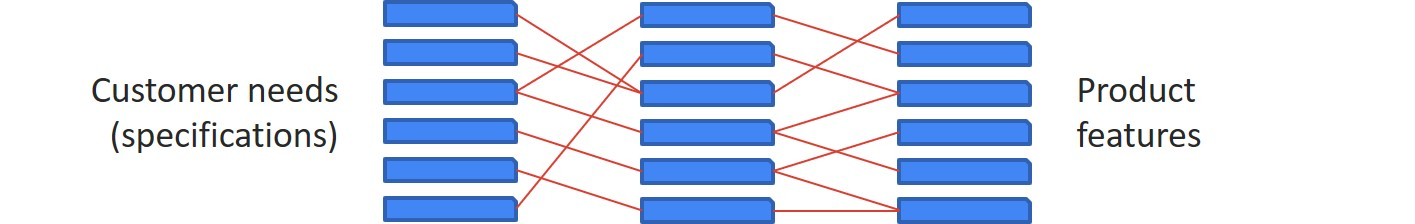
\includegraphics[]{traceability}
    \caption{Several connected requirements modeling the project traceability}
    \label{fig:mesh3}
\end{figure}
For more information about traceability, read our article about the traceability matrixes (it is in french but we will soon publish it in english).

\item[Author] : We will name the author, the person in charge of writing and updating the document thanks to the remarks on it.
\item[Reviewer(s)] : They are the people in charge of reading the document and commenting it to improve it before freezing the document and eventually sending it to the customer.
\item[Request For Proposal] : This is the document where the customer lists all the requirements describing his need.
\item[Specification] : A specification is the detailed description of an item of the solution. And so, what we call specifications is the document listing all the specifications matching the request for proposal.\\The name of such item or document may vary depending on the field of activity of one company. We chose to use them here as they are the most frequently used nouns we encountered.

